
In \cref{sec:resonator_spectroscopy_flux} we found a rough estimation of the sweetspot, exploiting the coupling between qubit and resonator.
The resonance frequency of the resonator changed (weakly) with the flux and we had to find the bias level that maximized it.\\
We now repeat a similar experiment with qubit spectroscopy, expecting to find a much more sensitive dependence between flux and qubit frequency.\\
The experiment is a bit of a merge between "Flux Resonator Spectroscopy" and "Qubit Spectroscopy":
\begin{itemize}
    \item we send a constant DC current at the qubit through the flux line. The voltage amplitude of this pulse will be the bias level;
    \item we perform a two-tone qubit spectroscopy;
    \item we repeat for different bias levels and different drive frequencies.
\end{itemize}
In respect to the experiments already executed, we can focus on much more narrow scans: in particular for the flux one of which we already have an estimation of the sweetspot.
Looking at \cref{fig:flux_resonator_spectroscopy_sketch}, for example, we could decide to focus our scan between $0.3$ and $0.5$. 
To obtain a sensible and overall \textit{good} plot, it is important to decrease the bias step; the effect of a too large step is visible in \cref{fig:qubit_spectroscopy_flux_sketch}.

\begin{figure}[ht]
    \centering
    \subfloat[\centering sufficiently fine step]{{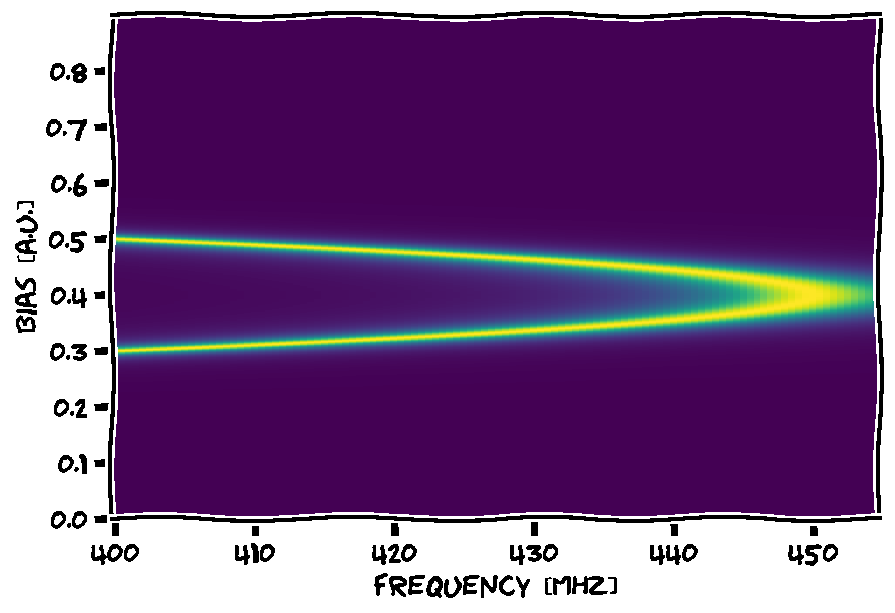
\includegraphics[width=6cm]{characterization/figures/qubit_spectroscopy_flux_sketch_good.pdf} }}%
    \qquad
    \subfloat[\centering too large step]{{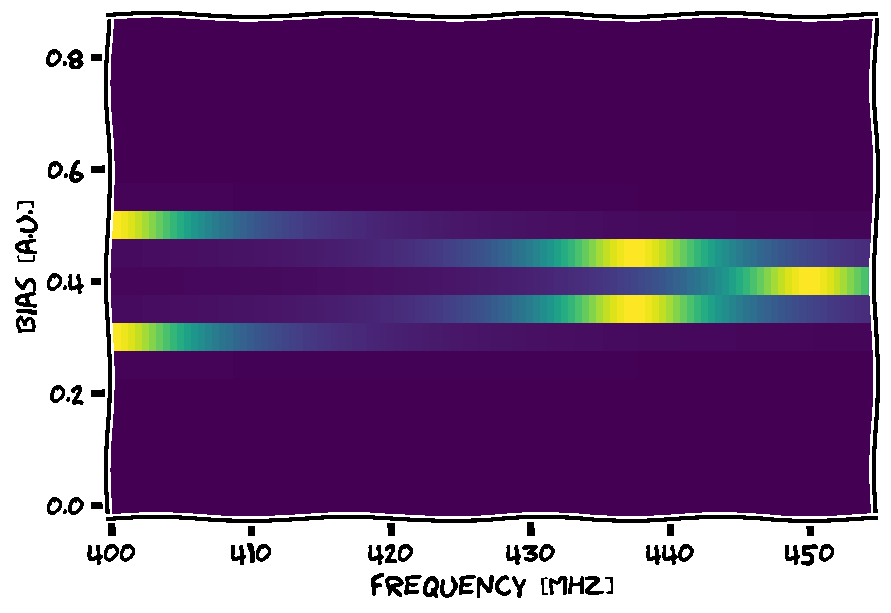
\includegraphics[width=6cm]{characterization/figures/qubit_spectroscopy_flux_sketch_bad.pdf} }}%
    \caption{Sketch of the plot expected for a flux qubit spectroscopy experiment with comparison between a "bad" and "good" step for the bias scan.}%
    \label{fig:qubit_spectroscopy_flux_sketch}%
\end{figure}

Another note on the parameter choices, in addition to all the ones that we already saw in the previous sections, we have here also the choice of the frequency span: in fact we already know the qubit frequency at the current estimation for the sweetspot and this can be the center of our scan, but how large should the scan be? 
This is extremely dependent on the qubit parameters and fabrication, but  we can say fro the beginning that the dependence will be much faster and steep than the one of the resonator.

It is useful to obtain a first realistic estimation of the parameters, to do an initial scan with larger steps (obtaining something like the first plot of \cref{fig:qubit_spectroscopy_flux_sketch}) to have a better idea of the strength of the qubit-flux dependence.

Some plots, for real case scenarios, are presented in \cref{fig:qubit_spectroscopy_new}.
Note that these plots come from acquisitions done at the same time, on qubits of the same chip (so manufactured with the same fabrication procedure) but nevertheless obtaining very different dependencies.

It is also important to repeat a \textit{caveat} already outlined in \cref{sec:resonator_spectroscopy_flux}: if the goal is to control multiple qubits at the same time, then this experiment \textit{must} be done at the same time for all the needed qubits. And, in particular, centering the sweetspots at the same time.


From these plots, we extract the sweetspot values as $0.753$, $0.022$ and $-0.01$.

After choosing the new sweetspot it may be worth to re-do resonator and qubit spectroscopies: the resonator one should not have changed much, but it is better to be sure; on the other hand, for sure the qubit one has changed, it is true that every information is already in the 3D plot, but a more straightforward visualization is helpful.

\begin{figure}[H]
    \centering
    \subfloat[\centering Qubit 0.]{
        \makebox[\textwidth][c]{
        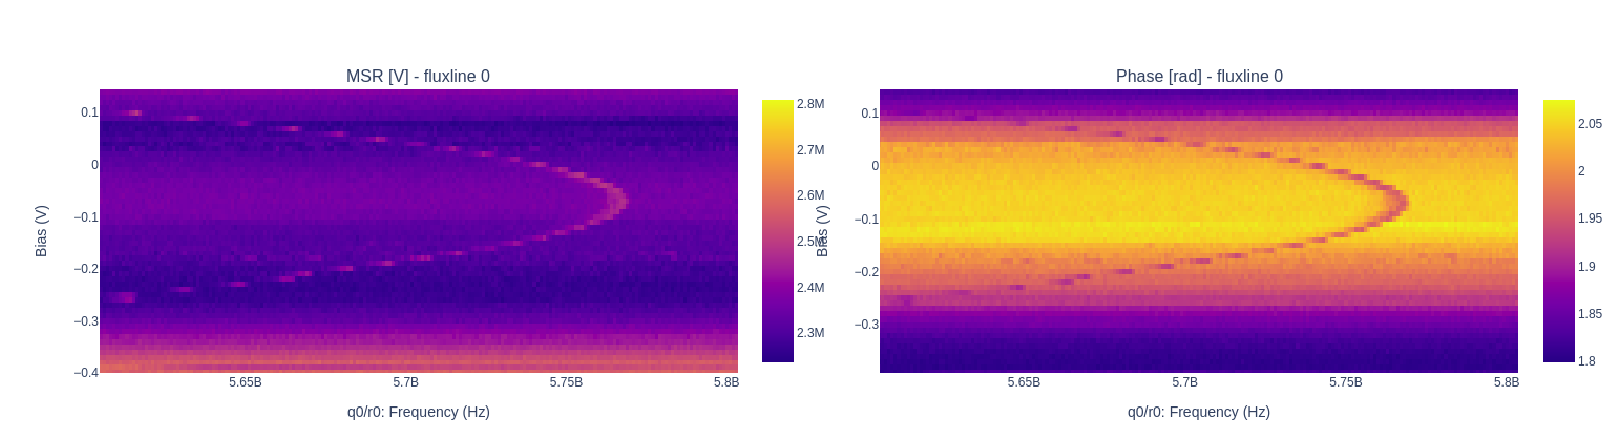
\includegraphics[width=0.87\textwidth]{characterization/figures/qubit_flux_spectroscopy.png}}
    }\\
    \subfloat[\centering Qubit 1.]{
        \makebox[\textwidth][c]{
        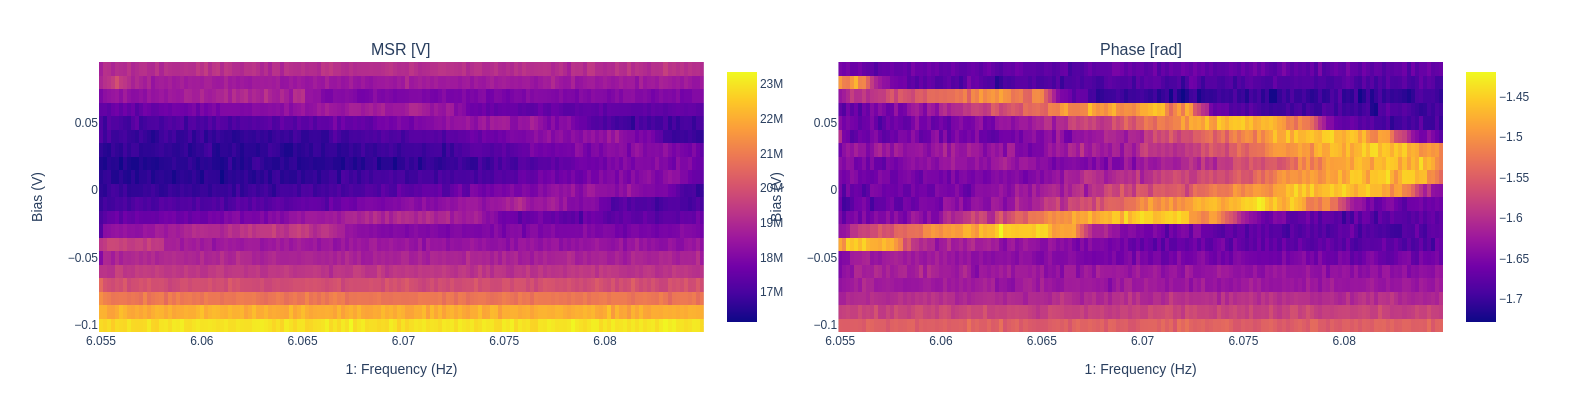
\includegraphics[width=0.9\textwidth]{characterization/figures/qubit_spec_flux_2.png}
        }
    }\\
    \subfloat[\centering Qubit 2.]{
        \makebox[\textwidth][c]{
        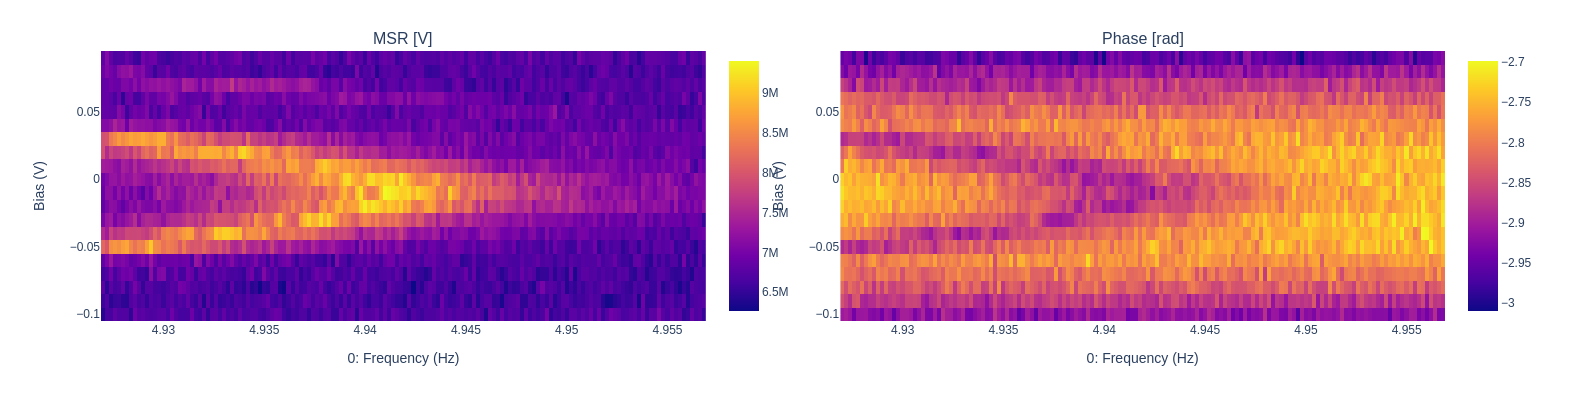
\includegraphics[width=0.9\textwidth]{characterization/figures/qubit_spec_flux_3.png}}
    }
    \caption{Plots for flux qubit spectroscopies.}
    \label{fig:qubit_spectroscopy_new}
\end{figure}

\fluxexperimentrecap
{Flux qubit spectroscopy}
{drive calibration, flux dependence calibration}
{flux sweetspot,\\qubit frequency at the sweetspot}
{a qubit spectroscopy experiment is executed for different frequencies and different biases (fixing the amplitude). We do a 3D plot with transmitted signal vs drive frequency vs bias. We extract bias and frequency for the sweetspot (highest frequency)}

